\documentclass[fleqn,11pt]{SelfArx} % Document font size and equations flushed left

\usepackage{placeins}

\setlength{\columnsep}{0.55cm} % Distance between the two columns of text
\setlength{\fboxrule}{0.75pt} % Width of the border around the abstract

\definecolor{color1}{RGB}{0,0,90} % Color of the article title and sections
\definecolor{color2}{RGB}{0,20,20} % Color of the boxes behind the abstract and headings

\newlength{\tocsep} 
\setlength\tocsep{1.5pc} % Sets the indentation of the sections in the table of contents
\setcounter{tocdepth}{3} % Show only three levels in the table of contents section: sections, subsections and subsubsections

%----------------------------------------------------------------------------------------
%	ARTICLE INFORMATION
%----------------------------------------------------------------------------------------

\JournalInfo{\ } % Journal information
\Archive{\ } % Additional notes (e.g. copyright, DOI, review/research article)

\PaperTitle{Advanced Computer Architecture: The ``Smooth'' Challenge} % Article title

\Authors{Romain Brault\textsuperscript{1}, Alexandre Camus\textsuperscript{2},  Giorgos Flourentzos\textsuperscript{3}} % Authors

\affiliation{\textsuperscript{1}RB812 \hfill \textsuperscript{2}AC5612 \hfill \textsuperscript{3}GF210}

\Keywords{} % Keywords - if you don't want any simply remove all the text between the curly brackets
\newcommand{\keywordname}{} % Defines the keywords heading name

%----------------------------------------------------------------------------------------
%	USEFULL TOOLS
%----------------------------------------------------------------------------------------

\usepackage[T1]{fontenc}
\usepackage[utf8]{inputenc}

\usepackage[english]{babel}

\usepackage{amsmath}
\usepackage{amsfonts}
\usepackage{amssymb}

\usepackage{enumerate}
\usepackage{caption}
\usepackage{subcaption}
\usepackage{listings}
\usepackage[pdftex=true,hyperindex=true,colorlinks=false,hidelinks]{hyperref}

% Fonts packages (if needed)
%\usepackage[nott,fullsumlimits]{kpfonts}
%\usepackage{lmodern}
\renewcommand{\ttdefault}{txtt}

\usepackage{cite}

%----------------------------------------------------------------------------------------
%	ABSTRACT
%----------------------------------------------------------------------------------------

\Abstract{Coding is a question of how to compute things, but also how to compute them the fastest. These are often two questions that can't be resolved at once. Although coding a program that gives the expected result is an obstacle, another problem arises when performance is to be maximized. Once this is done, optimizing the written code might take a lot of time, depending on whether the hardware on which it is running, is taken into account. Here, given a correct program, the aim was to optimize it, given a chosen architecture. This consisted of understanding the code, then optimizing it sequentially and finally trying to improve it by parallelizing through vectorization or offloading the calculation to an accelerator (GPU).}



% ---------------------------------------------------------------------------------------

\begin{document}


%----------------------------------------------------------------------------------------
%	LISTINGS OPTIONS
%----------------------------------------------------------------------------------------

\lstset{
basicstyle=\ttfamily,
keywordstyle=\color{blue},
identifierstyle=,
commentstyle=\color[rgb]{.2,.4,.5},
stringstyle=\ttfamily\color{gray},
breaklines=true}

%----------------------------------------------------------------------------------------

\flushbottom % Makes all text pages the same height

\maketitle % Print the title and abstract box

\tableofcontents % Print the contents section

\thispagestyle{empty} % Removes page numbering from the first page

%----------------------------------------------------------------------------------------

\section{Introduction}
\subsection{Context and Objectives}
\paragraph{}
Simulation in computer science is usually computationally intensive. Although an algorithm can be theoretically efficient\footnote{With a low complexity.}, a naive implementation, without any hardware consideration reveal to be slower than expected.

This paper start with a basic implementation of a curve smoothing algorithm where the curve -- a mesh -- is represented by a graph. This paper present a various methods to reduce the computation time of the smoothing algorithm on a specific machine, according to the hardware specification. The list of optimizations presented is non exhaustive, however the considered approach reduced the computation time by approximately 1300\% on the given architecture.

The method used to achieved this speed-up is the following:
\begin{itemize}  \vspace{-4mm}
\item first optimize on one CPU core, \vspace{-4mm}
\item then parallelize over one node (here a single computer), \vspace{-4mm}
\item eventually used hardware accelerator such as GPU.
\end{itemize}

\subsection{Software Considerations}
The hardware considered is one of the Imperial College computing laboratory. All these computer are equipped with an Intel CPU, thus the best performances were obtained using the Intel Compiler\footnote{The speed-up gained by switching from g++ (GNU) to icpc (Intel) is presented section \ref{}.}. However the Imperial College computer do not have the latest version of the Intel Compiler installed on, providing some optimizations and and the use of the new C++ standard (C++11). To obtained the maximum throughput additional library, not installed on Imperial College computer, such as blitz++, were used. A solution to have the best of the latest compiler version, library flexibility and the performances of the Imperial College computers is to cross-compile the code.

Cross-compiling is the action of creating executable code for a platform other than the one on which the compiler is running. This is challenging because the compiler usually tune the code to be as fast as possible on the machine where the code is compiled lowering the performances on the target machine. Additionally, extra care must be payed to the portability of the code.

The code was compiled on a Linux-Fedora 18 64bits station and is to run on a Linux-Ubuntu 12.04 64bits station.


\FloatBarrier
\subsection{Hardware Considerations}

Table \ref{CPUspecC} and \ref{CPUspecR} show respectively the hardware characteristics of the compiling machine and the running machine. The compiling machine is much slower than the running machine but is able to generate code optimized for the running machine.

\begin{table}[!h]
	\centering

	\begin{tabular}{|p{3.5cm}|p{4cm}|}
		\hline
		Model Name & Intel Core i7-QM720 \\
		\hline
		Clock Speed & 1.6 GHz \\
		\hline
		Max Turbo Frequency & 2.8 GHz \\
		\hline
		Cache line size and alignment & 64 B \\
		\hline
		CPU cores & 4 \\
		\hline
		CPU Threads & 8 \\
		\hline
		Integrated GPU & No \\
		\hline
		Memory Channels & 2 \\
		\hline
		Max Memory Bandwith & 21 GB/s \\
		\hline
		Flags & fpu, sse, sse2, sse3, ssse3, sse4\_1, sse4\_2 \\
		\hline
	\end{tabular}

	\caption{CPU Specifications for the compiling station.}
	\label{CPUspecC}
\end{table}

\begin{table}[!h]
	\centering

	\begin{tabular}{|p{3.5cm}|p{4cm}|}
		\hline
		Model Name & Intel Core i7-2600 \\
		\hline
		Clock Speed & 3.4 GHz \\
		\hline
		Max Turbo Frequency & 3.8 GHz \\
		\hline
		Cache line size and alignment & 64 B \\
		\hline
		CPU cores & 4 \\
		\hline
		CPU Threads & 8 \\
		\hline
		Integrated GPU & No \\
		\hline
		Memory Channels & 2 \\
		\hline
		Max Memory Bandwith & 21 GB/s \\
		\hline
		Flags & fpu, sse, sse2, sse3, ssse3, sse4\_1, sse4\_2, avx \\
		\hline
	\end{tabular}

	\caption{CPU Specifications for the running station.}
	\label{CPUspecR}
\end{table}

\paragraph{}
To summarize, the figure \ref{topo} gives a quick overview of the hardware topology. The GPU is connected on the PCI port \verb+10de:0618+.

\begin{figure}[h]
	\centering

	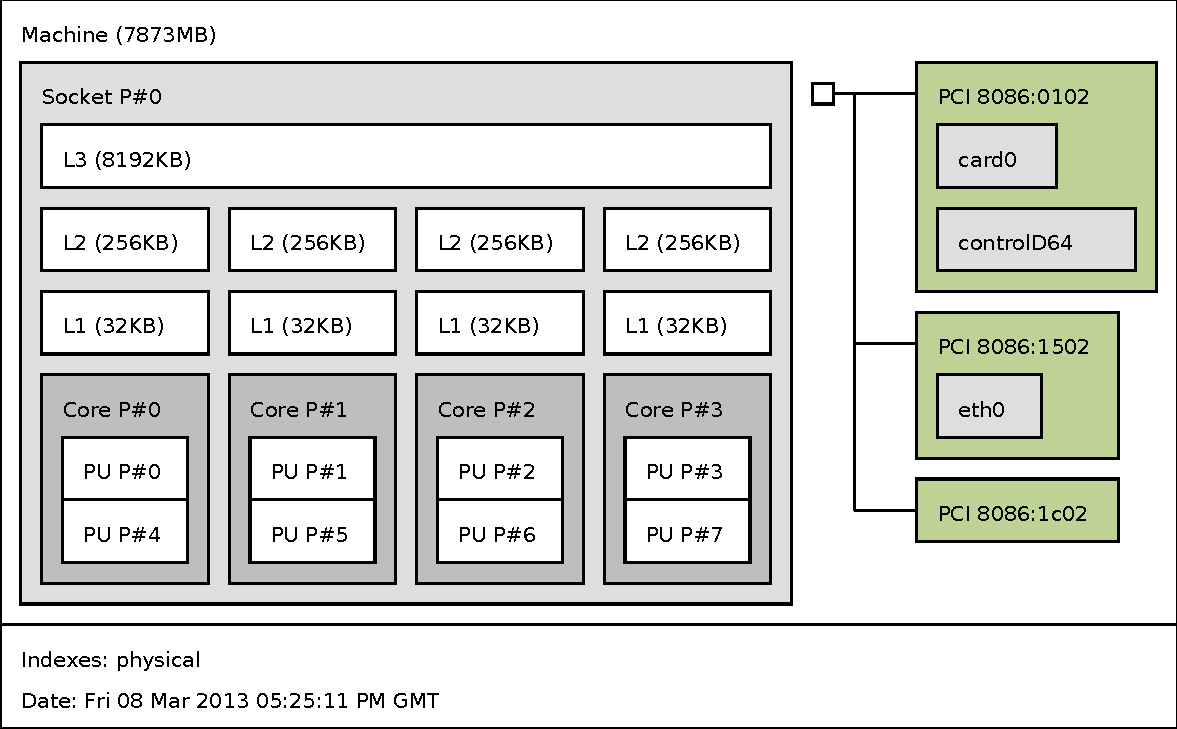
\includegraphics[width=.48\textwidth]{run.pdf}

	\caption{Topology of the running station.}
	\label{topo}
\end{figure}

\begin{figure}[h]
	\centering

	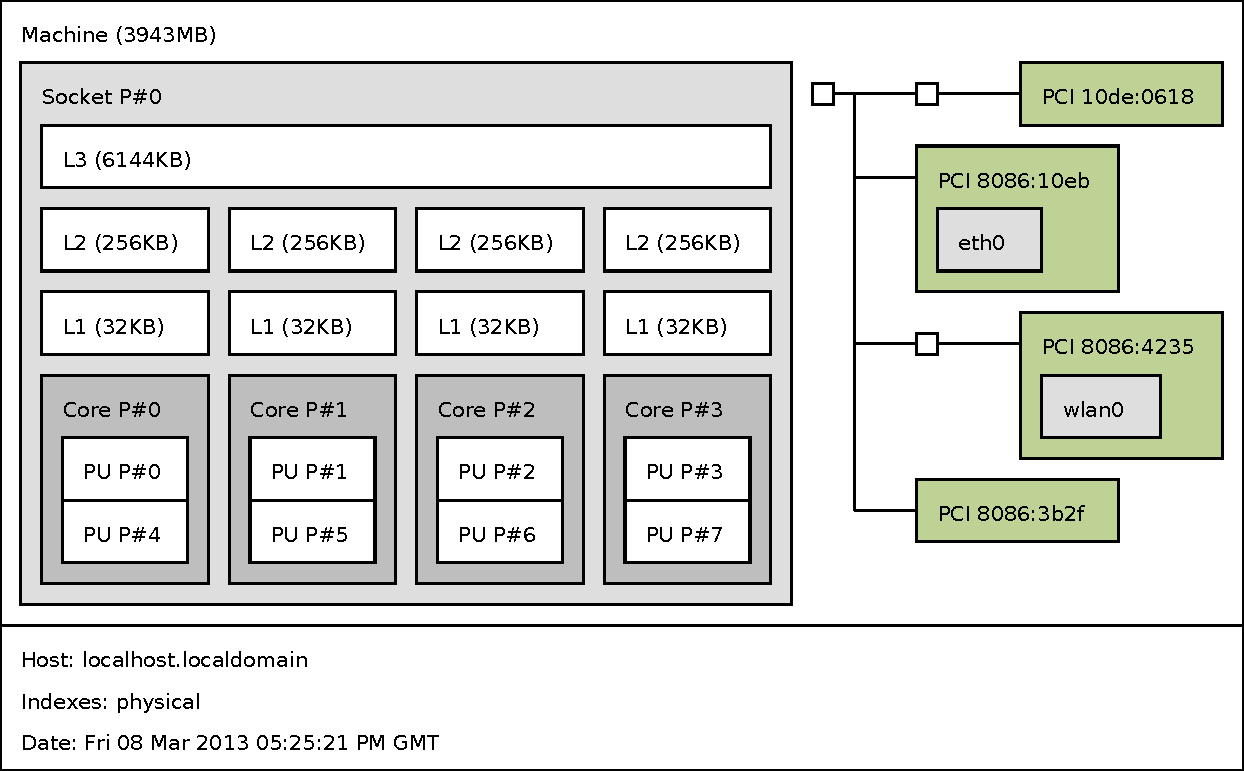
\includegraphics[width=.48\textwidth]{compile.pdf}

	\caption{Topology of the compiling station.}
	\label{topo}
\end{figure}


%----------------------------------------------------------------------------------------
\FloatBarrier
\section{The Sequential Issue}

After running for the first time the program, it appears that the method \verb+mesh_quality()+ is the most called and so is the most expensive in computation time. Hence its code has been considered as a potential source of optimization.

Reading the code, some sequential issues were found. There are three kinds of problems: the algorithms chosen, the coding style and the data's representation.

\subsection{Algorithm}

The method used to solve an equations' system was correct but two general to be efficient. The program needs only to solve systems of two equations in two unknowns. The Cramer's rule based on determinants is far more efficient.

The use of the method \verb+pow()+ seems a little too heavy in the method \verb+element_quality()+. As the number of multiplication is known, the use of simple multiplications is more efficient here, e.g. \verb+x*x*x+.

\subsection{Code Style}

Few changes in the style of the code might help the compiler. Some of these changes have been done to speed up the program.

Inline functions do often help the compiler to optimize the translated assembly language. That is why functions like \verb+isSurfaceNode()+ or \verb+isCornerNode()+ or \verb+element_quality()+ or \verb+svd_solve_2x2()+.

In loops changes have been made to avoid recomputation of the invariant (e.g. calling \verb+.size()+ in a loop). Instead, this invariant is now stored in a local variable.

\subsection{Data's Representation}

The data structure used is fine and one of the most efficient to represent a graph. However, the C++ structures used seem to be a little too big in this case. So instead of using vectors of sets, the program is now using vectors of vectors. This increases a little the global performance.

Similarly, the number of node does not exceed $10^5$ which is less than the maximum integer represented thanks to the \verb+uint32_t+. This type is faster to manipulate than the classic \verb+int+ type. Hence \verb+uint32_t+ has been preferred.

In the \verb+element_quality()+ method, the call of an element in a matrix during its multiplication, is very expensive in memory access. So instead of calling the element at each step of the loop, it is better to use an intermediate variable that is assigned into the matrix element at the end.

%----------------------------------------------------------------------------------------

\section{CPU Parallelization}

\subsection{Analysis}

Parallelization can't be done easily. The program needs to be slightly modified in order to cut the graph in groups of independent nodes. Independent nodes are nodes that can be inspected at the same time while running the program. To group nodes in such groups the graph must be colored. Then each color represents nodes that can be inspected at the same time because they are not adjacent.

But the coloring algorithm might be very expensive in computation time. This depends on the number of colors used and if this number is specified or not. In this very case, the goal of such an algorithm is to minimize the colors used in order to maximize parallel computations. Hence a powerful algorithm is needed.

\subsection{Optimization}

A first try was realized with a very basic algorithm that colors a graph without assuming anything on its structure. But the simple fact of coloring the graph was itself longer than the original program. This confirmed the need of a very powerful algorithm.

%----------------------------------------------------------------------------------------

\section{GPU Acceleration}

\subsection{Analysis}

%----------------------------------------------------------------------------------------

\section{Results}

\subsection{Sequential Improvements}

\subsection{Parallelization Performance}

\end{document}